\documentclass[10pt,a4paper]{article}
\usepackage[margin=0.68in,headheight=0pt,headsep=0pt]{geometry}
\usepackage[T1]{fontenc}
\usepackage[utf8]{inputenc}
\usepackage[spanish]{babel}
\usepackage{graphicx}
\usepackage{booktabs}
\usepackage{float}
\usepackage{xcolor}
\usepackage{enumitem}
\usepackage{microtype}

\setlength{\parindent}{0pt}
\setlength{\parskip}{3pt}
\setlength{\textfloatsep}{5pt}
\setlength{\intextsep}{4pt}
\setlength{\abovecaptionskip}{2pt}
\setlength{\belowcaptionskip}{0pt}
\renewcommand{\arraystretch}{1.04}
\setlist{nosep,leftmargin=*}
\pagestyle{plain}

\begin{document}

\begin{titlepage}
\thispagestyle{empty}
\centering
\vspace*{0.4cm}
% El logo de la UM va en prism-uploads/image.png; si falta, la carátula sale sin él.
\IfFileExists{prism-uploads/image.png}{\includegraphics[width=.60\textwidth,trim=0 1.5cm 0 1.1cm,clip]{prism-uploads/image.png}\par}{}
\vspace{0.3cm}
{\Large\color{blue!45!black} Facultad de Ingeniería\par}
\vspace{1.3cm}
{\large Curso de Inteligencia Artificial\\Tarea 2\par}
\vspace{1.0cm}
{\large Proyecto: Maceta Inteligente\par}
\vspace{1.6cm}
{\LARGE\bfseries\color{blue!45!black} Clasificador del estado de un lirio de paz en la ESP32\par}
\vspace{1.6cm}
{\large Manuel Pérez, Guillermo Storace y Phillip Bowles\par}
\vfill
{\large Octubre de 2026\par}
\end{titlepage}

\pagenumbering{arabic}
\section*{1. Objetivo, sistema y datos}
Se desarrolló un clasificador de tres estados para un lirio de paz, ejecutado localmente en una ESP32. Cada cinco minutos la placa lee una sonda resistiva de humedad del sustrato, un DHT11 (temperatura y humedad del aire) y un LDR; calcula las variables de entrada, predice y activa un LED: \texttt{saludable} (verde), \texttt{estresada} (amarillo) o \texttt{marchita} (rojo). Las muestras también se publican en un backend PostgreSQL. La inferencia no depende de WiFi.

El dataset de la Tarea 1, actualizado al 23/10/2026, contiene 21.850 registros de una maceta entre el 12/09 y el 22/10. Las etiquetas se anotan al observar la planta y se heredan hasta la observación siguiente, formando episodios. Se usó la hora NTP de la placa. Se remuestreó a cinco minutos mediante la mediana; se descartaron la primera hora tras cada reinicio, las lecturas saturadas y los registros sin etiqueta vigente. No se interpolaron huecos. El conjunto final reúne 5.663 filas en 24 episodios: 7 saludables, 11 estresados y 6 marchitos. Cuatro episodios dudosos se excluyeron del entrenamiento; la evaluación principal usa los 20 restantes.

\begin{figure}[H]
\centering
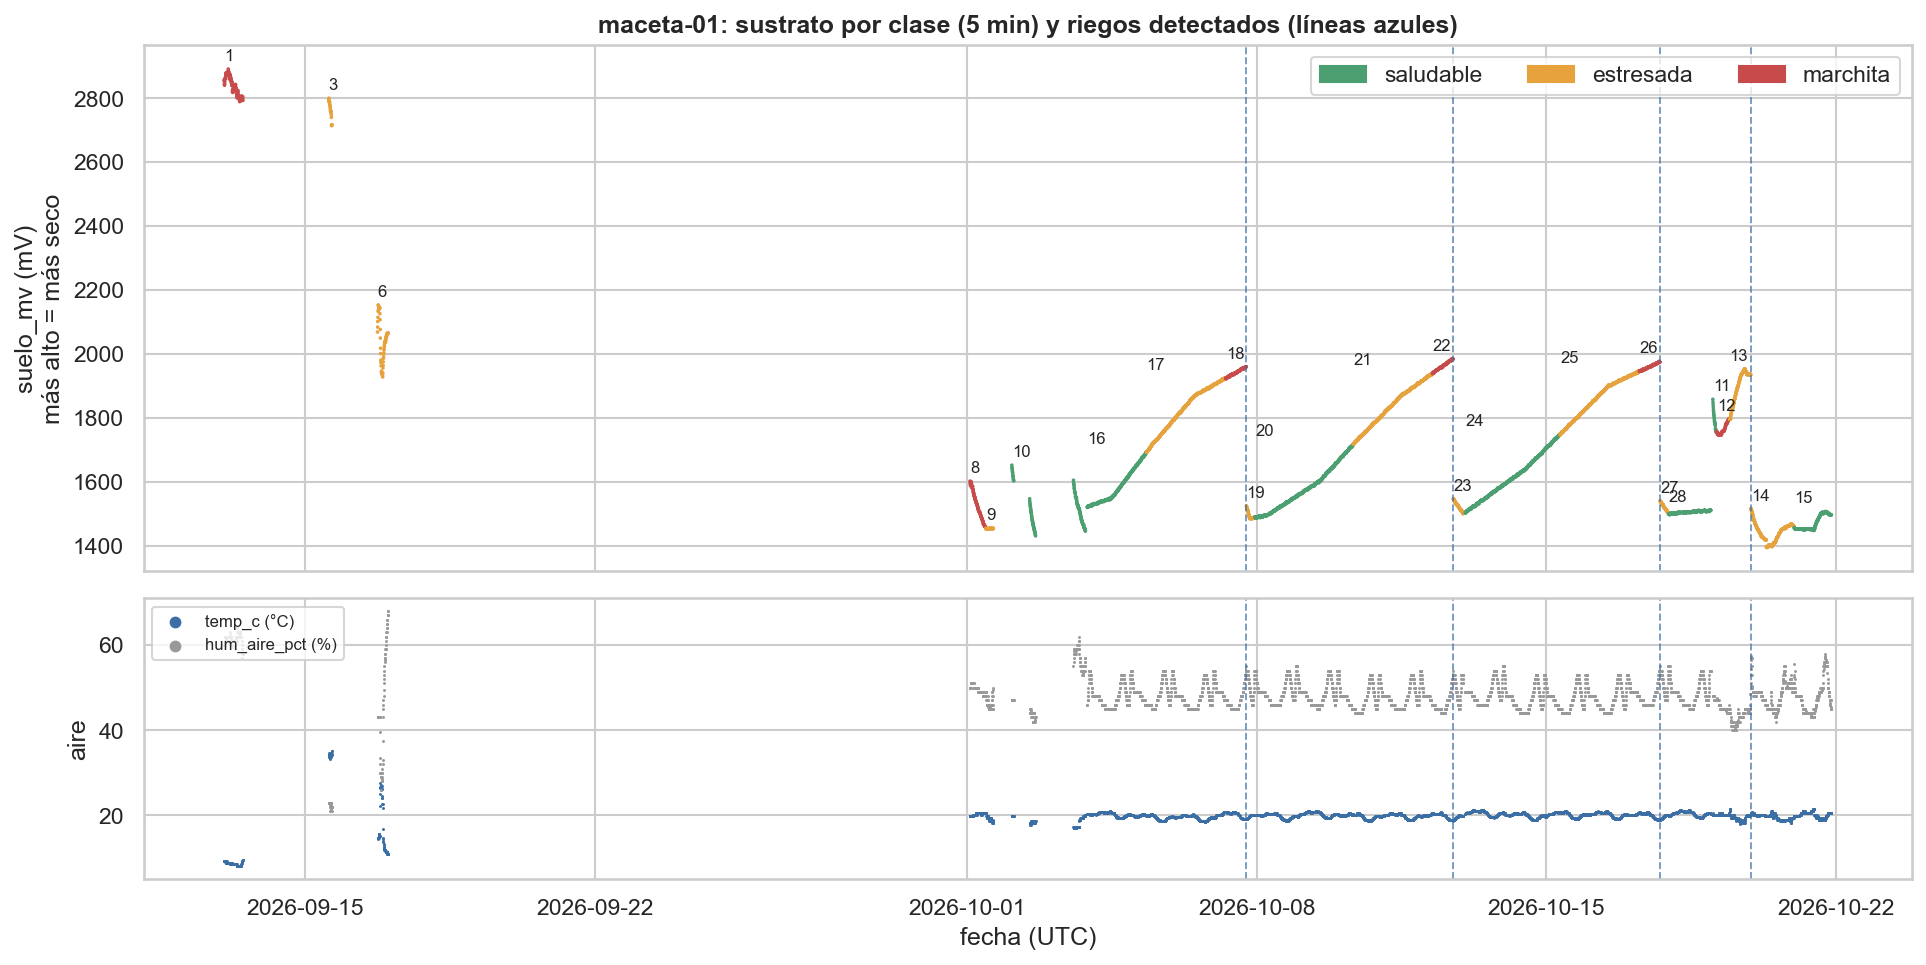
\includegraphics[width=.95\linewidth]{prism-uploads/serie_modelado.png}
\caption{Serie de modelado: humedad del sustrato por clase y riegos detectados (arriba), temperatura y humedad del aire (abajo). En octubre se distinguen tres ciclos de secado, marchitez, riego y recuperación. En la sonda, un valor mayor indica un sustrato más seco.}
\end{figure}

Las ocho variables calculadas con una ventana de 13 muestras son humedad actual y cambio del sustrato en una hora, temperatura, humedad del aire, VPD, luz actual y media horaria, y horas desde el último riego. La placa detecta el riego ante una caída de sonda de al menos 250 mV, fuera de la primera hora tras un reinicio, y guarda su instante en memoria no volátil. Se excluyó la luz porque confundía marchitez con mediciones nocturnas; tampoco se usaron columnas que revelan la etiqueta (episodio, origen u hora).

\clearpage
\section*{2. Evaluación y comparación}
Las muestras consecutivas son muy parecidas: un Random Forest alcanza 0,99 de exactitud balanceada con partición aleatoria, pero 0,75 al separar episodios. Para evitar fuga temporal se aplicó validación cruzada estratificada y agrupada por episodio, en cinco folds, con ajuste anidado de hiperparámetros. Se agregaron las predicciones fuera de fold y se estimó la variabilidad mediante bootstrap de episodios. Todos los candidatos usan la sonda y ninguno usa luz.

\textbf{Cuadro 1.} Resultados fuera de fold en los 20 episodios no dudosos; costo estimado en ESP32 a 240 MHz.
\begin{center}
\small
\begin{tabular}{@{}lrrrr@{}}
\toprule
Modelo & F1 macro & Exact. bal. & Recall marchita & Flash / $\mu$s\\
\midrule
\textbf{Regla sonda + riego} & \textbf{0,858 $\pm$ 0,049} & \textbf{0,860} & 0,77 & 111 B / 0,3\\
Dos umbrales (baseline) & 0,833 $\pm$ 0,057 & 0,834 & 0,77 & 8 B / 0,1\\
Árbol de decisión & 0,801 $\pm$ 0,055 & 0,815 & 0,74 & 111 B / 0,2\\
Regresión logística & 0,791 $\pm$ 0,057 & 0,827 & \textbf{0,85} & 52 B / 4\\
Random Forest (30 árboles) & 0,758 $\pm$ 0,075 & 0,753 & 0,56 & 6,1 KB / 11\\
k-NN & 0,744 $\pm$ 0,058 & 0,734 & 0,49 & 66 KB / 2.370\\
SVM RBF & 0,731 $\pm$ 0,077 & 0,756 & 0,66 & 12,5 KB / 981\\
MLP & 0,672 $\pm$ 0,079 & 0,663 & 0,30 & 1,1 KB / 26\\
Naive Bayes & 0,564 $\pm$ 0,090 & 0,561 & 0,14 & 60 B / 4\\
Clase mayoritaria (baseline) & 0,188 $\pm$ 0,089 & 0,203 & 0,00 & 4 B / 0\\
\bottomrule
\end{tabular}
\end{center}

\begin{figure}[H]
\centering
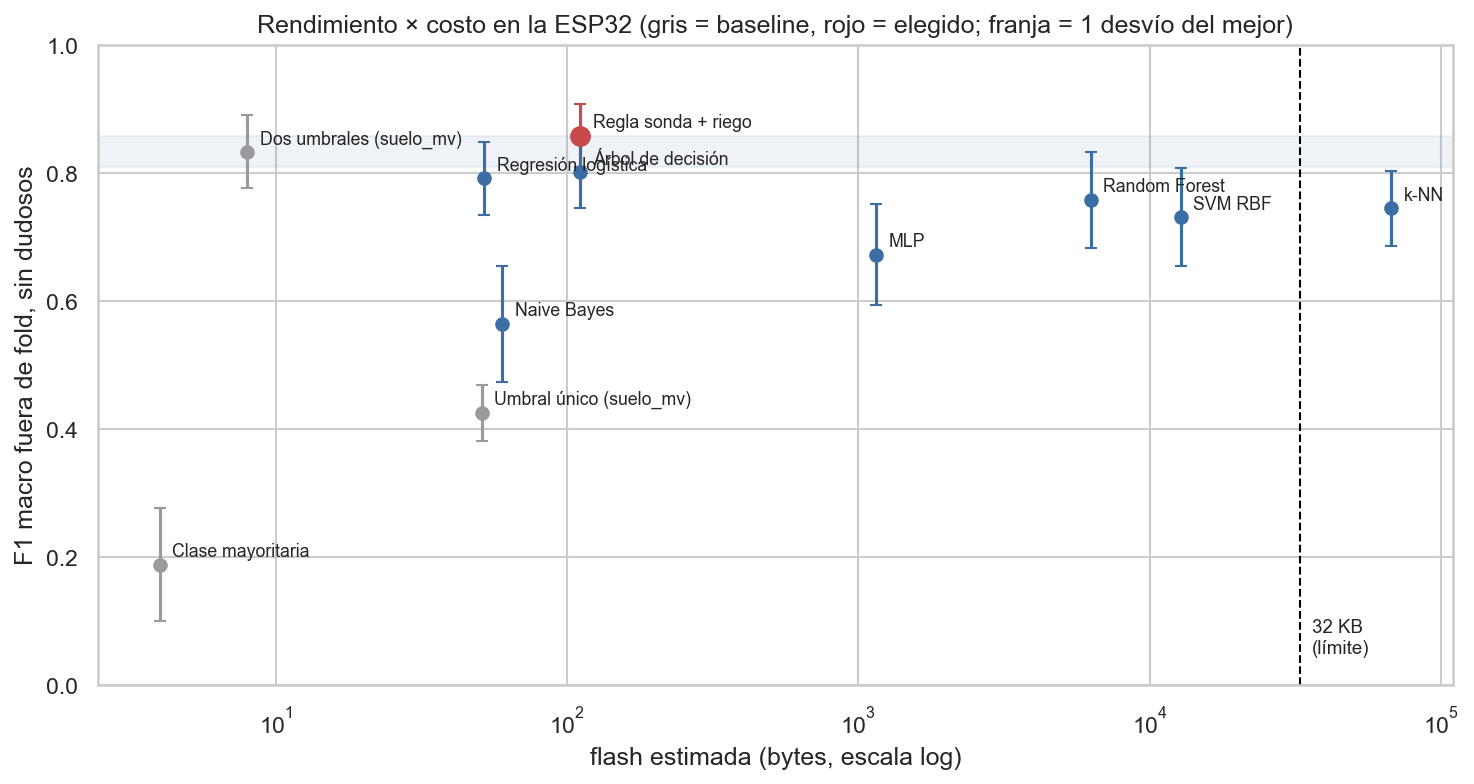
\includegraphics[width=.95\linewidth]{prism-uploads/rendimiento_vs_costo.png}
\caption{F1 macro fuera de fold frente a flash estimada (escala logarítmica). La franja indica un desvío del mejor resultado; la línea punteada marca el límite de 32 KB.}
\end{figure}

Las reglas simples superan a los modelos flexibles: 20 episodios aportan pocos ejemplos independientes. El aire tiene variación limitada en octubre (18--21\,$^\circ$C y 42--57\% de humedad); en un árbol, añadir humedad del aire elevó el F1 de 0,71 a 0,77, mejora posiblemente ligada al radiador de septiembre. La regla elegida combina buen desempeño, bajo costo e interpretabilidad.

\clearpage
\section*{3. Modelo, implementación y discusión}
La selección se fijó con tres criterios: menos de 32 KB de flash, menos de 1 ms por predicción y sin memoria dinámica; F1 macro a no más de un desvío del mejor (piso 0,809); y, en empate, interpretabilidad. La regla sonda + riego es la única que supera el piso y vence a la regla de dos umbrales y al árbol en 98\% y 99\% de las remuestras. En el conjunto con todos los episodios obtiene F1 macro 0,795 y ROC-AUC 0,83; esta cifra corresponde a una evaluación distinta de la tabla, que excluye episodios dudosos.

\begin{figure}[H]
\centering
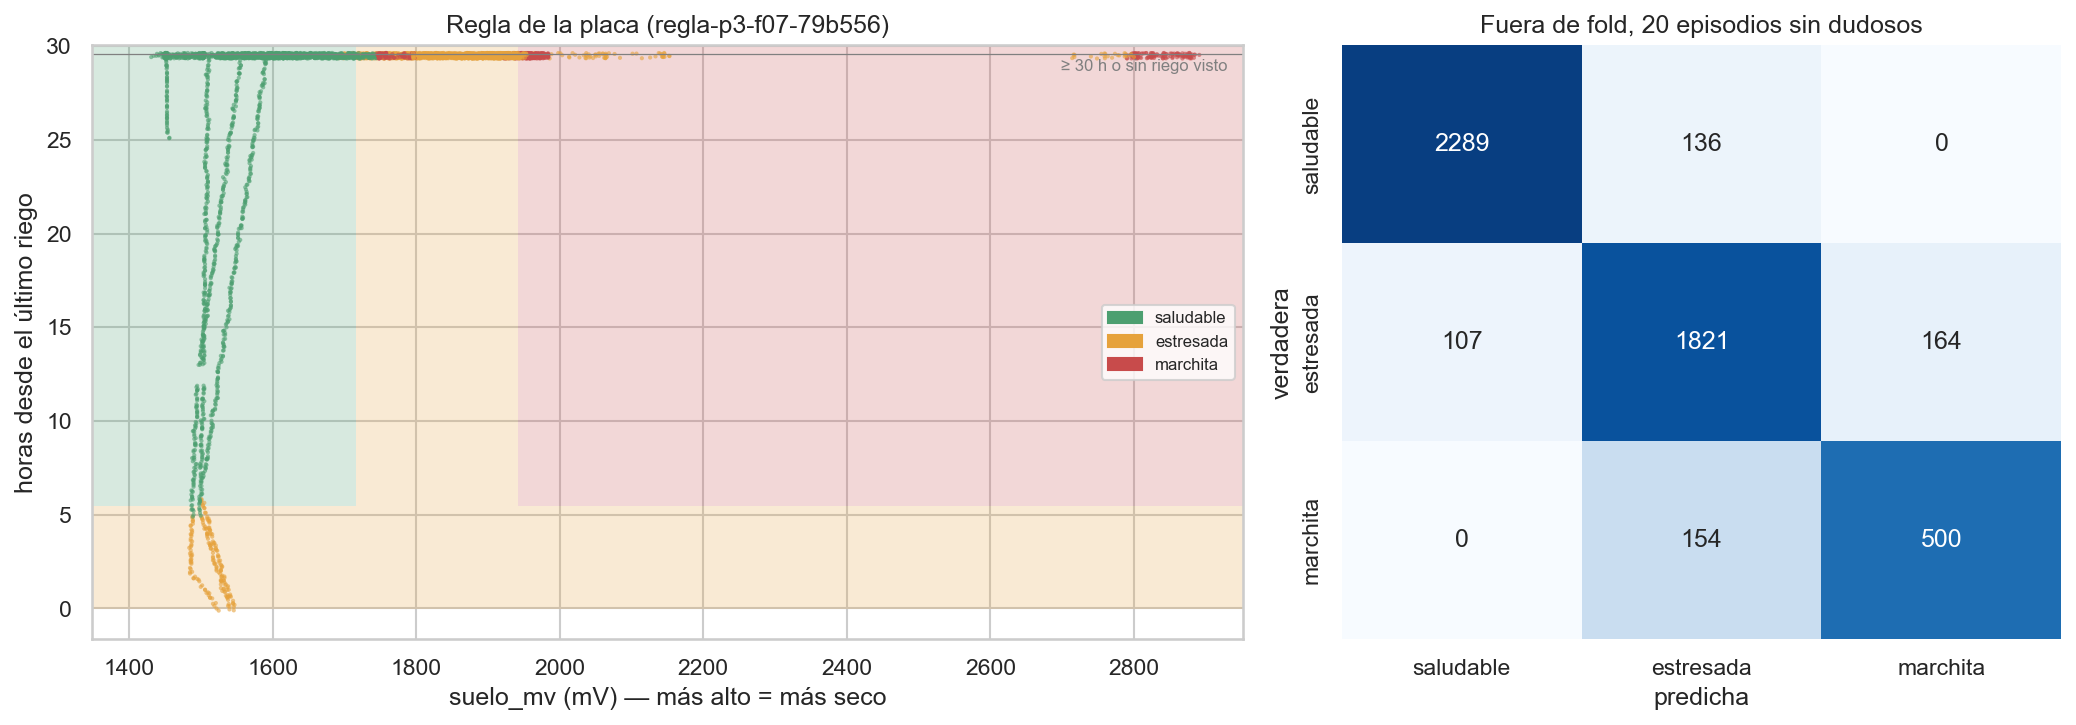
\includegraphics[width=.98\linewidth]{prism-uploads/modelo_final.png}
\caption{Regla de decisión en el plano humedad--tiempo desde el riego (izquierda) y matriz de confusión fuera de fold (derecha). No hay confusión directa entre saludable y marchita.}
\end{figure}

La función \texttt{plantaia\_predecir} (modelo \texttt{regla-p3-f07-79b556}) se exporta a tablas constantes en un encabezado C de 111 B y requiere como máximo tres comparaciones:
\begin{quote}\small\ttfamily
if (h\_desde\_riego <= 5.5) return ESTRESADA;\\
if (suelo\_mv <= 1716) return SALUDABLE;\\
if (suelo\_mv <= 1940) return ESTRESADA;\\
return MARCHITA;
\end{quote}

El firmware 2.1.0 lee sensores (mediana de nueve lecturas), actualiza el buffer circular, detecta riegos, arma las ocho variables, predice y controla el LED; luego envía clase, probabilidades y versión del modelo al backend. Si el DHT11 no respondió, omite la predicción y deja los LED apagados. Los 23 tests de host reportan paridad Python--C del 100\% en 336 vectores del modelo y 190 muestras de variables, incluidos umbrales, reinicios, huecos, faltantes y un riego.

El replay del 19/10 con el mismo código de la placa detectó una caída de 418 mV al regar a las 22:40. El log de host registra \texttt{n=171, h\_riego=5.5 -> ESTRESADA} y \texttt{n=172, h\_riego=5.6 -> SALUDABLE}. Es replay en host, no log serial de ejecución física. En operación, el modelo ocupa 111 B y predice en microsegundos; el firmware completo utiliza 73,5\% de flash (962 KB de 1,31 MB) y 14,6\% de RAM. Sobre 272 muestras sin etiqueta del 21--22/10 predijo saludable en todos los casos.

\textbf{Limitaciones y mejoras.} El umbral de 5,5 horas podría reflejar el horario de observación: solo se vieron tres recuperaciones. Trece episodios se concentran en dos semanas; además, la sonda resistiva deriva por corrosión (la lectura de marchitez pasó de unos 2.830 a 1.950 mV) y el modelo no reconoció una marchitez nocturna de 1.758 mV el 19/10. Las decisiones tomadas tras inspeccionar resultados pueden optimizar de más las métricas. Se propone observar recuperaciones en distintos horarios, calibrar semanalmente o usar una sonda capacitiva y evaluar predicciones junto con nuevas etiquetas guardadas en el backend.

\textbf{Agregado: detector por visión computacional.} Como segunda opinión, independiente de la sonda, el dashboard estima la turgencia a partir de una foto de la planta (de la ESP32-CAM o subida a mano) con visión clásica, sin aprendizaje. La imagen se lleva a 512 px y se segmenta el follaje con el índice de verdor ExG ($2G-R-B>25$ y $G>45$); tras un cierre morfológico se conserva sólo el componente conexo más grande, para descartar reflejos y otras plantas. La base de la planta es el borde de la maceta (la mancha terracota más grande debajo del follaje) o, si no se ve, el píxel verde más bajo de la franja central. Desde esa base se mide el ángulo medio de las hojas sobre la horizontal, llevado linealmente de 5$^\circ$ (0) a 70$^\circ$ (1), y el de las espatas, manchas blancas ($S<28$, $V>205$) junto a la planta, de 20$^\circ$ a 70$^\circ$. El puntaje es $100\,(0{,}6\,s_\mathrm{hojas}+0{,}4\,s_\mathrm{espatas})$, o sólo las hojas si no hay espatas visibles, y se traduce a las mismas clases que la placa: $\geq 67$ saludable, 34--66 estresada y $<34$ marchita. La respuesta incluye las métricas intermedias (ángulo de hojas y espatas, fracción del follaje que cuelga bajo la base y fracción verde) para auditar cada resultado. Se ajustó con cuatro fotos reales y tres sintéticas: en las reales dio 31, 0 y 9, frente a 20, 10 y 15 de un modelo de lenguaje con visión (Gemini). Depende del ángulo de la cámara y del color de la maceta, y por eso el dashboard guarda fotos etiquetadas para recalibrarlo.

\end{document}
